\documentclass[conference,leqno]{IEEEtran}
\IEEEoverridecommandlockouts
% Template version as of 6/27/2024

\usepackage{cite}
\usepackage{amsmath,amssymb,amsfonts}
\usepackage{algorithmic}
\usepackage{graphicx}
\usepackage{textcomp}
\usepackage{xcolor}
\usepackage{float}
\usepackage{array}
\usepackage[section]{placeins}

\def\BibTeX{{\rm B\kern-.05em{\sc i\kern-.025em b}\kern-.08em
T\kern-.1667em\lower.7ex\hbox{E}\kern-.125emX}}

\begin{document}

\title{Final Project: Few-Shot Detection of Bioacoustic Events}

\author{
\IEEEauthorblockN{Vicente Jos\'e Escarigo Miranda}
\IEEEauthorblockA{
\textit{UAM, Universidad Autonoma de Madrid} \\
\\
} }

\maketitle

\begin{abstract}
This report presents a lightweight few-shot bioacoustic event detection system
for DCASE 2023 Task 5. I use the official prototypical-network baseline model
and focus on feasible and valuable improvements without external data or
heavy backbones. Audio is converted to PCEN features with delta-MFCCs, encoded
by a shallow ResNet, and classified by distances to positive and negative
prototypes. This implementation uses adaptive segmentation at evaluation, negative sampling from
gaps between supports, transductive refinement of prototypes, and post-processing
rules. On the validation set, the proposed
model achieves 39.02\% F1 (precision 45.67\%, recall 34.06\%), improving
the official prototypical baseline by 9.43 absolute F1.
\end{abstract}

\begin{IEEEkeywords}
few-shot learning, bioacoustics, sound event detection.
\end{IEEEkeywords}


\section{Introduction}
Few-Shot Learning (FSL) is a ML approach that requires models to adapt to unseen classes using limited labeled examples. This is especially useful in cases where annotation is costly or time expensive. A common application is Sound Event Detection (SED), which identifies time boundaries of sounds in audio. In bioacoustics, recordings are frequently long with sparse positive events, making manual labeling difficult for which FSL proves to be useful by learning from minimal annotations.

The DCASE Task~5 challenge exemplifies this problem under several constraints: each file provides five support events, evaluation ignores all earlier content, and each file is processed independently \cite{dcasechallengeDCASE2023Task}. These rules emphasize obstacles like domain shifts, variable event durations, and noisy backgrounds.

This project builds on the official DCASE 2023 prototypical network baseline \cite{snellPrototypicalNetworksFewshot2017a}, aiming to improve it without external data or heavy modifications.
Although the 2024 edition introduces updated baselines and validation data, I use the 2023 version to ensure consistency with prior reports and isolate the impact of my modifications.
\section{State of the Art}
Prototypical Networks introduced an important development approach to few-shot
classification through metric learning, where the model is trained to map inputs
into an embedding space. In this space, classification is done by measuring the
distance to prototype representations of each class, resulting in
generalization from just a few labeled examples
\cite{snellPrototypicalNetworksFewshot2017a}. In 2022, most Task~5 systems stayed within
this template, improving the encoder, segmentation strategy, and post‑processing
\cite{liuSURREYSYSTEMDCASE2022,tangFEWSHOTEMBEDDINGLEARNING2022}. By 2023,
the best results came from frame‑level fine‑tuning,
(e.g., multi‑task branches) and from contrastive pretraining
\cite{yanMULTITASKFRAMELEVEL2023,moummadSUPERVISEDCONTRASTIVELEARNING2023}. In 2024, the
trend continued toward stronger backbones and pretraining (e.g., U‑Net variants
and AAPM‑style encoders), while prototypical methods were still strongly present
with important modifications like better negatives, attention mechanisms, or hybrid
front‑ends \cite{dengWeiLiu1Hy2024}.

\section{Description of the Proposed Method}

\subsection{Overview}
Firstly, audio is first converted into
time–frequency representations, embedded with a shallow ResNet encoder, and
evaluated through distance to class prototypes. Support positives form the
positive prototype, while negatives are sampled from regions between positive
events \cite{tangFEWSHOTEMBEDDINGLEARNING2022}. Query embeddings are scored
using softmax-based distances and converted to events. Figure~\ref{fig:pipeline}.

\FloatBarrier
\begin{figure}[H]
\centering
\includegraphics[width=0.65\columnwidth]{figs/pipeline.pdf}
\caption{Pipeline overview.}
\label{fig:pipeline}
\end{figure}

\subsection{Feature Representation}
I use a dual representation of PCEN and delta‑MFCCs to improve robustness
against channel and background variability. PCEN acts as a compressive, adaptive
gain control \cite{wangTrainableFrontendRobust2016}, while delta‑MFCCs capture
temporal dynamics \cite{hossanNovelApproachMFCC2011}. This combination provided
strong validation performance in DCASE 2022 Task 5
\cite{liuSURREYSYSTEMDCASE2022}.

\FloatBarrier
\begin{figure}[H]
\centering
\includegraphics[width=\columnwidth]{figs/fig_features_triplet.pdf}
\caption{Example input representations: log‑mel, PCEN, and delta‑MFCC.}
\label{fig:feature_triplet}
\end{figure}

\subsection{Segmentation}
I use fixed‑length patches during training (0.2\,s with 0.1\,s hop) so that all
episodes share a consistent input shape, this stabilizes episodic training. 
At evaluation time, I adapt the segment length per file
based on the \emph{maximum} duration among the five support events, using a rule
that shortens very long events while keeping enough temporal context. This follows the
Task~5 adaptive segmentation practice where evaluation windows track support duration
to avoid missing short calls or spreading long ones \cite{tangFEWSHOTEMBEDDINGLEARNING2022}.

\begin{equation}
\begin{aligned}
L &=
\begin{cases}
L_{\text{train}}, & \ell < L_{\text{train}} \\
\ell, & L_{\text{train}} \le \ell < L_{\text{lim}} \\
\lfloor \ell/2 \rfloor, & L_{\text{lim}} \le \ell \le 2L_{\text{lim}} \\
\lfloor \ell/4 \rfloor, & 2L_{\text{lim}} < \ell < 500 \\
\lfloor \ell/8 \rfloor, & \ell \ge 500
\end{cases} \\
H &= \max\!\big(1, \operatorname{round}(L/d)\big)
\end{aligned}
\label{eq:segmentation}
\end{equation}
where $\ell=\operatorname{round}(\max_i (t^{\text{end}}_i-t^{\text{start}}_i)\cdot f_s)$ is the
maximum support duration in frames, $L_{\text{lim}}$ is a length limit,
$L_{\text{train}}$ is the training segment length (in frames), and $d$ sets the hop
as a fraction of $L$. Equation~\eqref{eq:segmentation} is applied per file at
evaluation.

\subsection{Encoder Architecture}
I use a shallow ResNet encoder with three residual blocks (64–128–64 channels).
Deeper and more complex backbones can improve representations but are harder
to train with limited labeled segments. The original ProtoNet encoder uses 4
convolutional layers, making it vulnerable to vanishing gradients, which can
limit generalization \cite{yeFewShotLearningEmbedding2020}. I therefore adopt a
shallow ResNet‑18 variant that preserves skip connections and improves
optimization stability \cite{heDeepResidualLearning2016}. The residual block
structure is shown in Figure~\ref{fig:residual_block}, and the overall encoder
stages are summarized in Table~\ref{tab:resnet_stages}.

\FloatBarrier
\begin{figure}[H]
\centering
\includegraphics[width=0.85\columnwidth]{figs/residual_block.pdf}
\caption{Residual block used in the ResNet encoder.}
\label{fig:residual_block}
\end{figure}

\FloatBarrier
\begin{table}[H]
\caption{Encoder overview.}
\label{tab:resnet_stages}
\centering
\begin{tabular}{lcc}
\hline
\textbf{Layers} & \textbf{Channels} & \textbf{Kernel size} \\
\hline
ResidualBlock & 64 & 3$\times$3 \\
ResidualBlock & 128 & 3$\times$3 \\
ResidualBlock & 64 & 3$\times$3 \\
AdaptiveAvgPooling & -- & 4$\times$2 \\
\hline
\end{tabular}
\end{table}

\subsection{Training Method}
I train the encoder with episodic tasks, following the prototypical network
setup \cite{snellPrototypicalNetworksFewshot2017a}. Each episode samples
$C$ classes and draws $K$ support examples per class. The remaining 
examples from those classes form the query set.
Given support embeddings, class prototypes are computed as the mean of each
class (Eq.~\eqref{eq:proto}):
\begin{equation}
\mathbf{p}_{k}=\frac{1}{K}\sum_{i=1}^{K} f_\theta(\mathbf{x}^{k}_i)
\label{eq:proto}
\end{equation}
Each query embedding is classified by a softmax over negative squared
Euclidean distances to the prototypes (Eq.~\eqref{eq:proto_softmax}):
\begin{equation}
P(y=k \mid \mathbf{z}) =
\mathrm{softmax}\big(-d(\mathbf{z},\mathbf{p}_{1}),\ldots,-d(\mathbf{z},\mathbf{p}_{C})\big)_k
\label{eq:proto_softmax}
\end{equation}
The episode loss is the average negative log‑likelihood of the correct class
of all query examples. I reuse the same scoring rule at evaluation, where
the positive and negative prototypes are calculated from support and gap
segments, respectively. Figure~\ref{fig:episodic_training} illustrates the
episodic method used for training.

\FloatBarrier
\begin{figure}[H]
\centering
\makebox[\columnwidth][c]{\includegraphics[width=1.3\columnwidth]{figs/episodic_training.pdf}}
\caption{Episodic training schematic (C‑way (5), K‑shot (2)).}
\label{fig:episodic_training}
\end{figure}

\subsection{Transductive Refinement}
At evaluation I refine the prototypes using the unlabeled query embeddings. Starting
from $\mathbf{p}_{+}$ and $\mathbf{p}_{-}$, each query embedding $\mathbf{z}_i$ is softly
assigned to the two prototypes using negative distances:
\begin{equation}
\begin{aligned}
w_{i,+} &= \frac{\exp(-d(\mathbf{z}_i,\mathbf{p}_{+})/\tau)}{\exp(-d(\mathbf{z}_i,\mathbf{p}_{+})/\tau)+\exp(-d(\mathbf{z}_i,\mathbf{p}_{-})/\tau)} \\
w_{i,-} &= 1 - w_{i,+}
\end{aligned}
\label{eq:trans_assign}
\end{equation}
The query weighted updates are then computed and impact the current prototypes:
\begin{equation}
\begin{aligned}
\tilde{\mathbf{p}}_{+} &= \frac{\sum_i w_{i,+}\mathbf{z}_i}{\sum_i w_{i,+}}, \quad
\tilde{\mathbf{p}}_{-} = \frac{\sum_i w_{i,-}\mathbf{z}_i}{\sum_i w_{i,-}} \\
\mathbf{p}_{\pm} &\leftarrow \frac{\mathbf{p}_{\pm} + \lambda \tilde{\mathbf{p}}_{\pm}}{1+\lambda}
\end{aligned}
\label{eq:trans_update}
\end{equation}
where $\tau$ controls the confidence of the assignments and $\lambda$ is the query weight.
This update is repeated for a fixed number of iterations and 
adapts the prototypes to the test file without labels \cite{boudiafFewShotSegmentationMetaLearning2021}. 
Earlier versions of my implementation
showed large file-to-file variance, due to difficulty adapting the prototypes to each specific recording.
In respect to this, this step was fundamental.

\subsection{Post‑Processing Logic}
Event predictions are refined using heuristic filtering. Short events are
removed, and close detections are merged to avoid double detections.
Thresholds for duration and gap filtering are obtained based on the average
positive event duration
\cite{hertkornFEWSHOTBIOACOUSTICEVENT2022}:
\begin{equation}
\begin{aligned}
\text{keep event} &:\ (t^{\text{end}}-t^{\text{start}}) \ge \alpha\,\bar{t} \\
\text{merge if} &:\ (t^{\text{start}}_{i+1}-t^{\text{end}}_{i}) \le \beta\,\bar{t}
\end{aligned}
\label{eq:postproc}
\end{equation}

\section{Experimental Setup}

\subsection{Dataset overview}
To develop this project, I used the DCASE 2023 Task5 development set
\cite{dcasechallengeDCASE2023Task}. The Training Set contains five subsets
(BV, HT, JD, MT, WMW) with event annotations, consisting of 174 recordings,
21,h, 47 classes, and 14,229 positive events. Event ratio varies between
0.04--0.24, and sampling rates vary between 6--48,kHz. The Validation Set
contains three subsets (HB, PB, ME) with 18 recordings and 1,034 positive
events, and event ratio of 0.01--0.7, as well as sampling
rates 44.1--48,kHz. There is no class overlap between training and validation.
Table~\ref{tab:train_overview} and Table~\ref{tab:val_overview} summarize these
splits.

\FloatBarrier
\begin{table}[H]
\caption{Training set overview.}
\label{tab:train_overview}
\centering
\begin{tabular}{lcccc}
\hline
\textbf{Subset} & \textbf{Recordings} & \textbf{Duration} & \textbf{Classes} & \textbf{Events} \\
\hline
BV  & 5   & 10\,h        & 11 & 9\,026 \\
HT  & 5   & 5\,h         & 3  & 611 \\
JD  & 1   & 10\,m        & 1  & 357 \\
MT  & 2   & 1\,h\,10\,m  & 4  & 1\,294 \\
WMW & 161 & 4\,h\,40\,m  & 26 & 2\,941 \\
\hline
\textbf{Total} & \textbf{174} & \textbf{21\,h} & \textbf{47} & \textbf{14\,229} \\
\hline
\end{tabular}
\end{table}

\FloatBarrier
\begin{table}[H]
\caption{Validation set overview.}
\label{tab:val_overview}
\centering
\begin{tabular}{lcccc}
\hline
\textbf{Subset} & \textbf{Recordings} & \textbf{Duration} & \textbf{Classes} & \textbf{Events} \\
\hline
HB & 10 & 2\,h\,38\,m & 1 & 712 \\
PB & 6  & 3\,h        & 2 & 260 \\
ME & 2  & 20\,m       & 2 & 62 \\
\hline
\textbf{Total} & \textbf{18} & \textbf{5\,h\,57\,m} & \textbf{5} & \textbf{1\,034} \\
\hline
\end{tabular}
\end{table}

\subsection{Protocol and Annotations}
Validation uses a 5-shot protocol. Only the first five positive events in each
file are used as support. Evaluation ignores data before the fifth event ends.
Unknown (UNK) segments are excluded.

\subsection{Feature Extraction}
Audio is resampled to 22.05\,kHz. 128-bin mel spectrograms are computed with
$n\_fft=512$ and hop=256. PCEN is applied, and 40-dimensional delta‑MFCCs are
concatenated, following Task~5 settings shown to work well in other similar systems
\cite{wangTrainableFrontendRobust2016,hossanNovelApproachMFCC2011,liuSURREYSYSTEMDCASE2022}. This results in
168 features per frame, so each segment is shaped $(T,F)=(17,168)$ and batched as
$(B,17,168)$ before entering the encoder.

\subsection{Model Training}
Training segments are 0.2\,s with 0.1\,s hop. The encoder is trained for 10
epochs with 2000 episodes per epoch using Adam ($\mathrm{lr}=10^{-3}$) and a
StepLR scheduler (step size 10, gamma 0.5). Validation accuracy selects the best
checkpoint.

\subsection{Evaluation Configuration}
During evaluation, segment length is adapted per file using
Eq.~\eqref{eq:segmentation} with $L_{\text{lim}}=20$ frames, hop divisor $d=2$, and
$L_{\text{train}}=17$ as a lower bound. Negative prototypes are averaged from 30
samples over 6 iterations. Transductive refinement follows
Eq.~\eqref{eq:trans_assign}--\eqref{eq:trans_update} for 2 steps
($\tau=1.0$, $\lambda=0.1$). Post‑processing uses the rules in
Eq.~\eqref{eq:postproc} with threshold 0.6, $\alpha=0.2$, and $\beta=0.05$.

\subsection{Evaluation Metric}
Performance is measured with the official macro-averaged F-measure using
event-based IoU and bipartite matching. Support regions are excluded \cite{DcasefewshotbioacousticEvaluation_metricsMain}.

\section{Experiments and Results}
In order to optimize the configuration, I ran several grid searches across
different parameters to attempt improvements.
These include post‑processing parameters (minimum duration and merge gap
fractions), negative sampling (samples per iteration and iteration count), hop
divisor, segment‑length limit, transductive refinement parameters
($\tau$, $\lambda$, steps), and threshold sweep. For which the optimal
values found were stated in the previous section.

\begin{figure}[!ht]
\centering
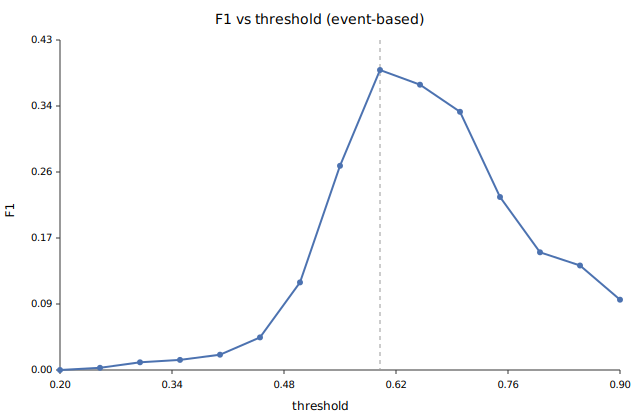
\includegraphics[width=\columnwidth]{figs/f1_vs_threshold.pdf}
\caption{Validation F1 as a function of threshold. The best F1 occurs at 0.6.}
\label{fig:f1_thresh}
\end{figure}

Transductive refinement modifies the positive and negative prototypes toward the
query distribution, while keeping a high cosine similarity between them.
An example on ME1 is reported in Table~\ref{tab:trans_refine}.
\begin{table}[!ht]
\caption{Example of transductive refinement on ME1 (changes
per step ($\tau=1.0$, $\lambda=0.1$)).}
\label{tab:trans_refine}
\centering
\begin{tabular}{lccccc}
\hline
\textbf{Step} & \textbf{$\Delta p_{+}$} & \textbf{$\Delta p_{-}$} & \textbf{$\|p_{+}\|$} & \textbf{$\|p_{-}\|$} & \textbf{cos$(p_{+},p_{-})$} \\
\hline
Init & 0.000 & 0.000 & 7.597 & 8.016 & 0.966 \\
0 & 0.176 & 0.109 & 7.616 & 8.026 & 0.970 \\
1 & 0.166 & 0.099 & 7.638 & 8.037 & 0.974 \\
\hline
\end{tabular}
\end{table}
\FloatBarrier

Validation performance against the two official baselines and the 2023 winning
system shows that post‑processing and transductive refinement both contribute to
the final score (Table~\ref{tab:results}). Their combined use reults in the best performance,
reaching an F1 of 39.02\%
with precision 45.67\% and recall 34.06\%. This is a +9.43 absolute F1
improvement over the official prototypical baseline and far above the
template‑matching baseline, though it remains below state‑of‑the‑art results.

Per class precision, recall, and F1 are reported in
Table~\ref{tab:subset_results}. Performance varies by file: ME and HB recordings
tend to be detected more reliably, while PB files with very short events and dense
activity resulted lower recall. This is somewhat to be expected due to the known sensitivity of
segment‑level methods to event duration and annotation density \cite{hertkornFEWSHOTBIOACOUSTICEVENT2022,tangFEWSHOTEMBEDDINGLEARNING2022,liuSURREYSYSTEMDCASE2022}.

\begin{table}[!ht]
\caption{Validation performance compared to official baselines and the 2023 winner.}
\label{tab:results}
\centering
\renewcommand{\arraystretch}{1.15}
\begin{tabular}{p{4.3cm}ccc}
\hline
\textbf{Method} & \textbf{Precision} & \textbf{Recall} & \textbf{F1} \\
\hline
Template Matching (baseline) & 2.42 & 18.32 & 4.28 \\
Prototypical Network (baseline) & 36.34 & 24.96 & 29.59 \\
Du et al. (2023 winner) \cite{yanMULTITASKFRAMELEVEL2023} & 76.20 & 75.30 & 75.70 \\
\hline
NO post-processing + NO transductive refinement & 41.97 & 28.68 & 34.08 \\
Post-processing only & 45.31 & 28.28 & 34.82 \\
Transductive refinement only & 42.74 & 34.33 & 38.08 \\
\textbf{Proposed model} & \textbf{45.67} & \textbf{34.06} & \textbf{39.02} \\
\hline
\end{tabular}
\end{table}


\begin{table}[!ht]
\caption{Validation Per-subset performance.}
\label{tab:subset_results}
\centering
\begin{tabular}{lccc}
\hline
\textbf{Subset} & \textbf{Precision} & \textbf{Recall} & \textbf{F1} \\
\hline
HB & 64.86 & 54.08 & 58.98 \\
ME & 43.12 & 90.38 & 58.39 \\
PB & 36.94 & 25.79 & 30.37 \\
\textbf{Overall} & \textbf{45.67} & \textbf{34.06} & \textbf{39.02} \\
\hline
\end{tabular}
\end{table}

\section{Discussion and Conclusion}
The experiments show that the official prototypical baseline can be significantly improved
with the inclusion of several lightweight modifications and finetuning. 
The largest sensitivity comes from post‑processing
threshold choice and minimum‑duration filtering. The gap between subsets
are an example of the limitations of segment‑level matching on short, dense events (PB),
where a frame‑level model or stronger temporal modeling would probably help.
Transductive refinement stabilizes file‑to‑file variance, but is limited
by the quality of the encoder and the negative sampling strategy \cite{boudiafFewShotSegmentationMetaLearning2021,tangFEWSHOTEMBEDDINGLEARNING2022}.

In conclusion, I implemented a few‑shot bioacoustic event detection pipeline that
improves the DCASE 2023 prototypical baseline by 9.43 F1 points on the validation
set. This implementation could be further improved through many ways, such as 
frame‑level processing, self‑supervised pretraining with allowed data, more complex embedding
backbones, or multi‑task learning.
\bibliographystyle{IEEEtran}
\bibliography{references}

\end{document}
